%%%%%%%%%%%%%%%%%%%%%%%%%%%%%%%%%%%%%%%%%%%%%%%%%%%%%%%%%%%%%%%%%%%
%%% Documento LaTeX 																						%%%
%%%%%%%%%%%%%%%%%%%%%%%%%%%%%%%%%%%%%%%%%%%%%%%%%%%%%%%%%%%%%%%%%%%
% Título:		Capítulo 1
% Autor:  	Ignacio Moreno Doblas
% Fecha:  	2014-02-01, actualizado 2019-11-11
% Versión:	0.5.0
%%%%%%%%%%%%%%%%%%%%%%%%%%%%%%%%%%%%%%%%%%%%%%%%%%%%%%%%%%%%%%%%%%%
% !TEX root = A0.MiTFG.tex
\chapterbegin{Fundamentos teóricos sobre propagación de pulsos ultracortos}
\label{chp:ManLaTeX}
\minitoc

\begin{sinopsis}
\label{sec:chpltx:sinop}
En este capítulo se presentan los fundamentos teóricos necesarios para analizar la propagación de pulsos ópticos ultracortos en medios no guiados, con especial atención a la atmósfera y al océano. En primer lugar, se introducen conceptos básicos de óptica como la longitud de onda, el índice de refracción, la constante de propagación, la dispersión y las ventanas de transmisión. A continuación, se describen las propiedades específicas de los pulsos ultracortos, sus formas temporales más habituales, el papel de la frecuencia instantánea y el efecto \textit{chirp}, así como la influencia de la velocidad de grupo y de la dispersión cromática en su ensanchamiento. Por último, se estudian los fenómenos de turbulencia atmosférica y oceánica y las principales herramientas estadísticas de canal empleadas para caracterizarla, como la función de coherencia mutua y la irradiancia promedio. Estos contenidos constituyen la base conceptual sobre la que se construye el modelo matemático de propagación desarrollado en el capítulo siguiente.
\end{sinopsis}

\section{Conceptos básicos de óptica}
Esta sección introduce los conceptos fundamentales necesarios para comprender la propagación óptica en distintos medios. Se describen magnitudes básicas como la longitud de onda, el índice de refracción y la constante de propagación, así como el papel de la dispersión y las ventanas de transmisión en la atmósfera y el océano.

\subsection{Longitud de onda}
La longitud de onda ($\lambda$) se define como la distancia entre dos crestas consecutivas de una onda en un instante de tiempo concreto\cite{España}. Matemáticamente, se relaciona con la frecuencia ($f$) y la velocidad de la luz en el vacío ($c$) mediante:
\begin{equation}
\lambda = \frac{c}{f}.
\label{eq:lambdacnu}
\end{equation}
En la práctica, la mayoría de las fuentes ópticas no son perfectamente monocromáticas, sino que presentan una banda estrecha de frecuencias alrededor de un valor medio. En este caso, se habla de radiación cuasimonocromática, y la longitud de onda de referencia se toma como la longitud de onda central asociada a esa frecuencia media. A mayor frecuencia corresponde una longitud de onda menor, y viceversa \cite{España}. Este concepto resulta fundamental en comunicaciones ópticas, ya que la atenuación, la dispersión cromática y los efectos de turbulencia dependen fuertemente de la longitud de onda empleada en la transmisión.

\subsection{Índice de refracción}
El índice de refracción ($n$) es un parámetro fundamental para describir el comportamiento de la luz en distintos medios materiales. Se define como la razón entre la velocidad de la luz en el vacío ($c$) y la velocidad de fase ($v_\mathrm{f}$) en el medio considerado mediante la siguiente formulación\cite{España}:
\begin{equation}
n = \frac{c}{v_\mathrm{f}}.
\label{eq:n-c-vf}
\end{equation}
Cuanto mayor es el índice de refracción de un material, más se reduce la velocidad de la luz al propagarse en él. El valor mínimo de este parámetro es uno, correspondiente al vacío, donde la luz alcanza su máxima velocidad. De este modo, el índice de refracción indica cuánto se ralentiza la luz dentro de un material y determina, además, el grado de desviación o refracción que experimenta al atravesar la frontera entre dos medios \cite{Britannica}.

\subsection{Constante de propagación}
La propagación de una onda en un medio puede describirse mediante la denominada constante de propagación. Físicamente indica cuántas oscilaciones de la onda caben por metro en la dirección de propagación. En medios guiados, como la fibra óptica, se asume que la luz se propaga principalmente en una única dirección, lo que simplifica el análisis. En cambio, en propagación no guiada, como en el océano o la atmósfera, la onda se distribuye en varias direcciones, lo cual hace el análisis de la propagación más complejo \cite{España}.


En la práctica, las señales ópticas reales no están compuestas por una única frecuencia, sino por un conjunto de componentes espectrales próximas entre sí, lo que lleva a describir la propagación mediante parámetros que pueden depender de la frecuencia. De forma general, la propagación puede describirse mediante una constante de propagación compleja dependiente de la frecuencia angular $\omega$, que puede expresarse como:
\begin{equation}
\gamma(\omega) = \alpha(\omega) + \mathrm{j}\beta(\omega),
\end{equation}
donde $\alpha(\omega)$ es la constante de atenuación del medio y $\beta(\omega)$ es la constante de fase. El término $\alpha(\omega)$ tiene en cuenta las pérdidas del medio y provoca una disminución de la amplitud del pulso durante la propagación, mientras que $\beta(\omega)$ gobierna la evolución de la fase del campo óptico\cite{ScienceDirect}.

\subsection{Medio dispersivo}
Un medio dispersivo es aquel en el que la velocidad de propagación de la luz depende de su frecuencia. Dicho de otro modo, las diferentes componentes espectrales de una onda no viajan a la misma velocidad, sino que cada una experimenta un retardo distinto, lo que provoca distorsiones temporales y ensanchamiento de la señal. Este fenómeno se conoce como dispersión y se manifiesta especialmente en pulsos ultracortos, cuyo ancho espectral es amplio y hace más notoria la diferencia de retardos. La fibra óptica constituye un ejemplo clásico de medio dispersivo, pero también lo son la atmósfera terrestre y el océano \cite{España}.

\subsection{Ventanas de transmisión}
En comunicaciones ópticas, no todas las longitudes de onda se propagan con la misma eficiencia. Existen regiones del espectro conocidas como ventanas de transmisión, donde la atenuación y la dispersión son menores y, por tanto, la propagación resulta más favorable.

En el caso de la atmósfera, las ventanas de transmisión se sitúan en el infrarrojo cercano, en torno a \SI{850}{\nano\meter} y \SI{1310}{\nano\meter}. Sin embargo, la ventana más relevante es la de \SI{1550}{\nano\meter}, ya que combina la menor atenuación (\textnormal{$\approx$} \SI{0.2}{\deci\bel\per\kilo\meter}) con una dispersión reducida\cite{España}. Además, esta longitud de onda coincide con la banda de operación de los sistemas de fibra óptica facilitando la compatibilidad entre enlaces guiados y no guiados.

La atenuación atmosférica depende en gran medida de las condiciones meteorológicas. En presencia de niebla, lluvia o polvo, los fenómenos de absorción y dispersión aumentan significativamente las pérdidas. La dispersión Rayleigh afecta principalmente a longitudes de onda cortas, mientras que en el infrarrojo cercano resulta casi despreciable. En cambio, en condiciones de niebla o bruma, donde predominan partículas de tamaño comparable a la longitud de onda, la dispersión Mie se convierte en el factor dominante \cite{Trichili}. 

En la práctica, la atenuación atmosférica para una longitud de onda dada se modela principalmente como un efecto de dispersión de Mie. Para estimar cuantitativamente dicha atenuación a lo largo de un enlace de distancia, se emplea habitualmente el modelo de Kim de 1999, que expresa la pérdida en función de la longitud de onda utilizada y de la visibilidad del entorno.

En todos los escenarios, la longitud de onda de \SI{1550}{\nano\meter} es la que presenta el comportamiento más robusto, como se observa en la Tabla~\ref{Tabla1}.

\begin{table}[H]
\centering
\setlength{\tabcolsep}{10pt}
\renewcommand{\arraystretch}{1.2}
\begin{tabular}{lccc}
 & & \multicolumn{2}{c}{\textbf{Atenuación [dB/km]}} \\
\cline{3-4}
\textbf{Condición atmosférica} & \textbf{Visibilidad [km]} & \textbf{850 nm} & \textbf{1550 nm} \\
\hline
Aire limpio        & 23   & 0.42  & 0.20 \\
Neblina            & 4    & 2.8   & 1.6  \\
Bruma              & 2    & 6     & 4    \\
Niebla ligera      & 1    & 13    & 9    \\
Niebla moderada    & 0.5  & 28    & 21   \\
Niebla densa       & 0.2  & 73    & 60   \\
Niebla muy densa   & 0.05 & 309   & 272  \\
\hline
\end{tabular}
\caption{Atenuación atmosférica para longitudes de onda de 850 nm y 1550 nm bajo distintas condiciones meteorológicas. Adaptado de \cite{Trichili}}
\label{Tabla1}
\end{table}


En el océano, la situación es distinta debido a la absorción molecular del agua y a la dispersión provocada por partículas, fitoplancton y detritos (véase Figura~\ref{Figura1}). En aguas claras o moderadamente turbias, se ha demostrado que la ventana azul-verde (\SIrange{450}{550}{\nano\meter}) es la más adecuada, ya que ofrece la menor absorción del agua y, por tanto, permite mayores distancias de transmisión. Además, esta ventana proporciona un ancho de banda útil del orden de los \si{\mega\hertz}, lo que la hace especialmente adecuada para aplicaciones de comunicaciones ópticas submarinas. Sin embargo, en aguas muy turbias la dispersión en esas longitudes puede ser crítica resultando más ventajoso recurrir a longitudes de onda más cercanas al rojo o infrarrojo cercano. Aunque la absorción es mayor, la dispersión se reduce \cite{Sun}.

\begin{figure}[H]
  \centering
  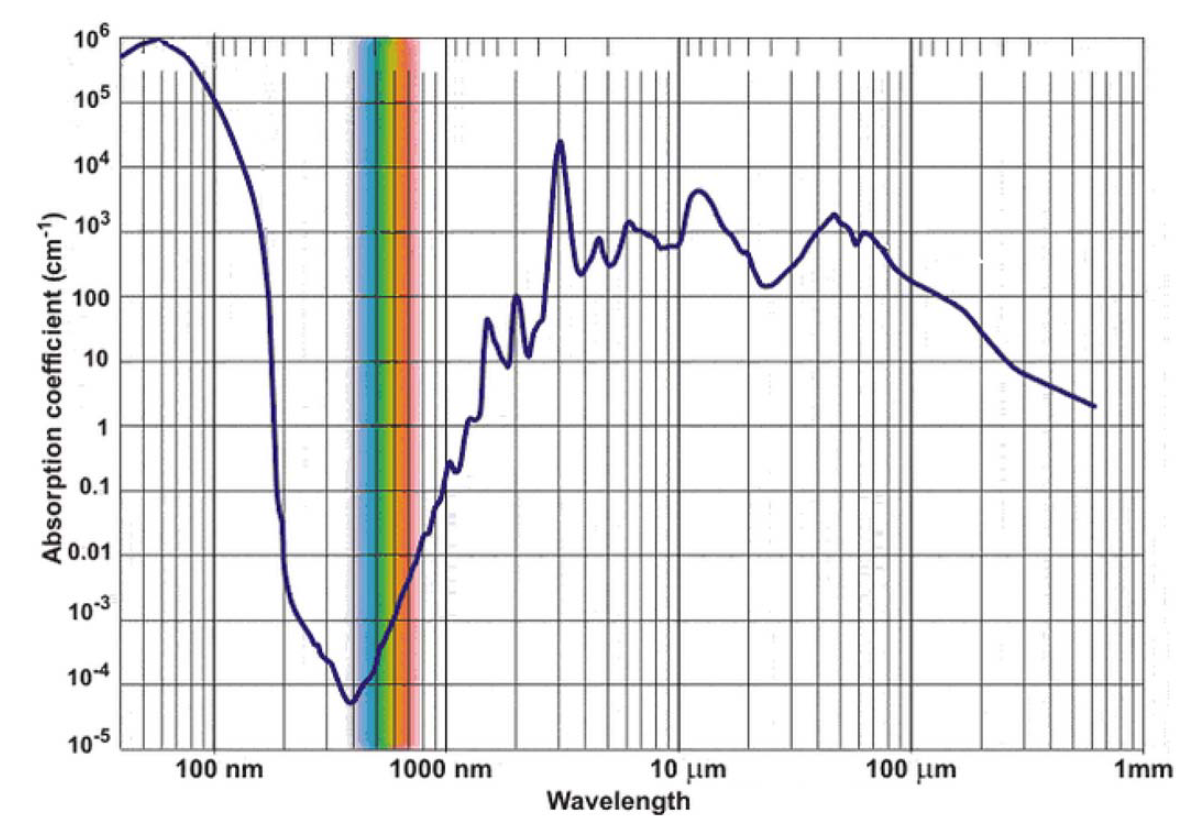
\includegraphics[width=0.7\linewidth,keepaspectratio]{figuras/Figura1.png}
  \caption{Coeficiente de absorción del agua en función de la longitud de onda. Fuente: \cite{Chaplin}}
  \label{Figura1}
\end{figure}

\section{Propagación y dispersión de pulsos ultracortos}
Esta sección aborda la descripción y el comportamiento de los pulsos ópticos ultracortos al propagarse por medios dispersivos. Se presentan sus formas temporales más habituales, el papel de la frecuencia instantánea y del efecto \textit{chirp}, así como la influencia de la velocidad de grupo, la dispersión cromática y el desarrollo de la constante de propagación en el ensanchamiento y la distorsión de los pulsos.

\subsection{Pulsos ultracortos}
Un pulso óptico puede entenderse como un breve destelleo de luz generado por un láser u otro dispositivo relacionado. Estos presentan un notable potencial para la generación de pulsos de luz con propiedades especiales. Gracias a la diversidad de técnicas disponibles, es posible producir pulsos con duraciones que abarcan desde ns hasta fs, lo que abre la puerta a aplicaciones muy variadas, que van desde las telecomunicaciones hasta la metrología ultraprecisa.

Los pulsos ópticos se emiten habitualmente en forma de haz láser de alta coherencia espacial, lo que asegura una propagación en una dirección bien definida y permite focalizarlos en áreas muy reducidas, a veces inferiores a \SI{1}{\micro\meter\squared}. La combinación de un foco pequeño y una duración ultracorta conduce a intensidades ópticas muy elevadas, aun cuando la energía total del pulso no sea grande \cite{Paschotta}. 
Los pulsos ópticos ultracortos pueden describirse como una onda portadora de alta frecuencia modulada por una envolvente de variación mucho más lenta como se observa en la Figura~\ref{Figura2}.

\begin{figure}[H]
  \centering
  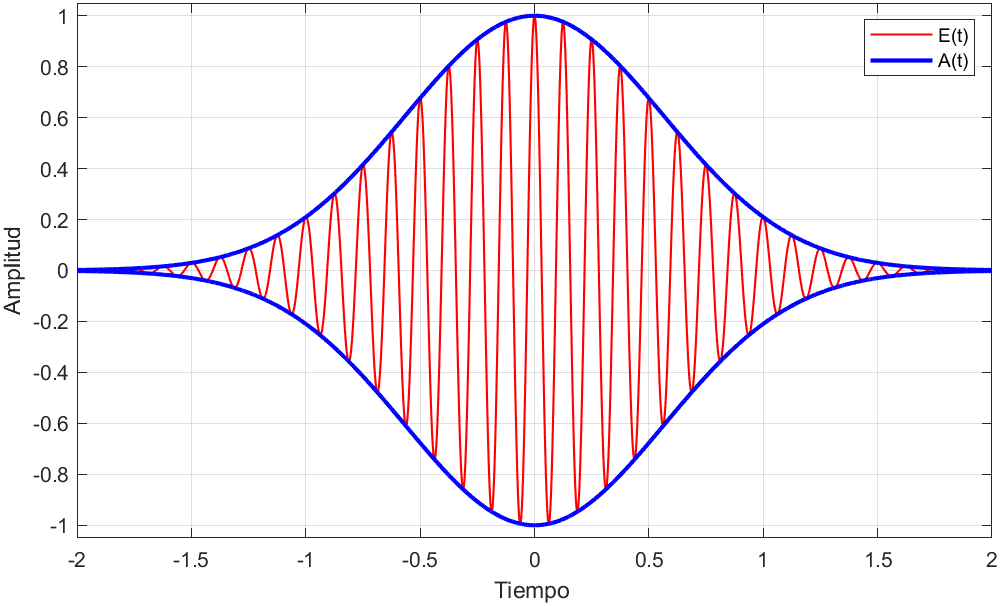
\includegraphics[width=0.8\linewidth,keepaspectratio]{figuras/Figura2.png}
  \caption{Representación de un pulso ultracorto: campo eléctrico ${E(t)}$ (curva roja) y su envolvente ${A(t)}$ (curva azul). Las magnitudes representadas son adimensionales y se emplean con fines ilustrativos}
  \label{Figura2}
\end{figure}

Una consecuencia directa de su corta duración es que presentan un espectro muy ancho: cuanto más breve es un pulso en el tiempo, mayor es el rango de frecuencias que lo compone, lo que constituye una manifestación del principio de incertidumbre tiempo-frecuencia \cite{Paschotta}. Esta propiedad juega un papel fundamental en el comportamiento de los pulsos ultracortos y motiva la necesidad de describirlos mediante modelos matemáticos adecuados, que se introducirán en las secciones siguientes.


\subsection{Formas de pulso: gaussiano, hiperbólico-secante y supergaussiano}
En este trabajo se consideran tres formas habituales de pulsos ópticos ultracortos: el pulso gaussiano, el pulso hiperbólico-secante y el pulso supergaussiano. En particular, el análisis y las simulaciones desarrolladas se centran en el pulso gaussiano, por tratarse del caso de referencia más empleado en la literatura y por permitir una caracterización analítica clara de los efectos de ensanchamiento y distorsión. No obstante, se incluyen también el pulso hiperbólico-secante y el supergaussiano como perfiles igualmente habituales en el ámbito de la óptica ultrarrápida, con el objetivo de presentar brevemente sus definiciones y facilitar posibles extensiones futuras del modelo a otras formas de pulso. Las expresiones y definiciones empleadas para describir las formas de pulso presentadas en esta subsección se basan en la formulación recogida en \cite{Agrawal}.


\subsubsection{Pulso gaussiano}
Un pulso gaussiano puede describirse, en el origen de la propagación, mediante la siguiente expresión\cite{Marcuse}:
\begin{equation}
U(0,T) = \exp\left(-\frac{T^{2}}{2T_{0}^{2}}\right),
\end{equation}
donde $U(0,T)$ representa la envolvente temporal del pulso, $T$ es el tiempo retardado respecto al centro del pulso y $T_{0}$ es el parámetro de duración temporal, definido como la semianchura del pulso en el punto $1/e$ de la envolvente. En la práctica, la duración del pulso suele caracterizarse mediante la \acs{FWHM}~(\acl{FWHM}), relacionada con $T_{0}$ por: \begin{equation}
T_{\mathrm{FWHM}} = 2\sqrt{\ln 2}\,T_{0} \approx 1.665\,T_{0}.
\end{equation}
Para incluir la posibilidad de que el pulso presente una variación temporal de su frecuencia instantánea, se introduce un parámetro de \textit{chirp}, $C$, de modo que la expresión del pulso en el origen adopta la forma \cite{Agrawal}:
\begin{equation}
U(0,T) = \exp\left[-\frac{(1+iC)T^{2}}{2T_{0}^{2}}\right].
\end{equation}
El parámetro $C$ controla la variación lineal de la frecuencia instantánea a lo largo del pulso, sin alterar su envolvente temporal inicial.

Finalmente, la siguiente figura muestra la envolvente temporal del pulso gaussiano.

\begin{figure}[H]
  \centering
  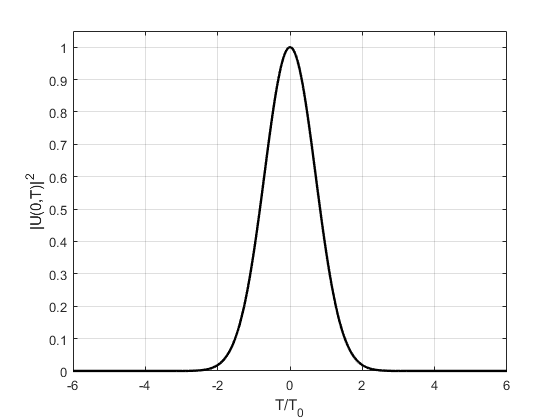
\includegraphics[width=0.6\linewidth]{figuras/PulsoGaussiano.png}
  \caption{Envolvente temporal normalizada de un pulso gaussiano en el origen de la propagación con $C=0$}
  \label{gaussiano_z0}
\end{figure}

\subsubsection{Pulso supergaussiano}
Una extensión de los pulsos gaussianos la constituyen los pulsos supergaussianos, empleados para modelar señales con bordes más abruptos, como los emitidos por láseres semiconductores modulados directamente. Matemáticamente se describen en el origen como \cite{Potasek}:
\begin{equation}
U(0, T) = \exp\left[-\frac{1 + iC}{2} \left(\frac{T}{T_{0}}\right)^{2m}\right],
\end{equation}
donde $T_{0}$ es el parámetro temporal característico, $C$ es el \textit{chirp} inicial y $m$ controla la abrupta transición de los bordes. Para un valor de $m=1$ se recupera el caso gaussiano, mientras que valores mayores generan pulsos con forma más cuadrada y bordes más pronunciados. Esta mayor abrupticidad se traduce en un espectro más ancho, lo que hace a estos pulsos especialmente sensibles a los efectos dispersivos.

Finalmente, la siguiente figura muestra la envolvente temporal del pulso supergaussiano.

\begin{figure}[H]
  \centering
  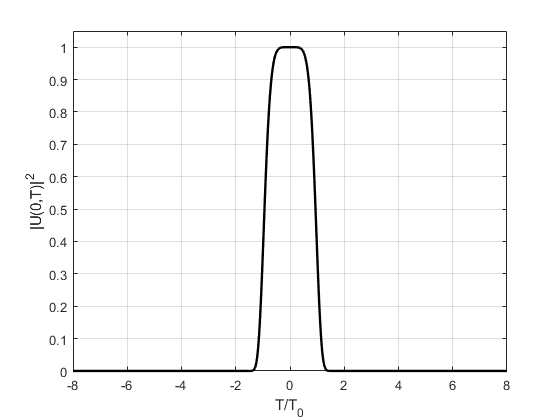
\includegraphics[width=0.6\linewidth]{figuras/PulsoSuperGauss.png}
  \caption{Envolvente temporal normalizada de un pulso supergaussiano en el origen de la propagación con $C=0$ y $m=3$}
  \label{supergaussiano_z0}
\end{figure}


\subsubsection{Pulso hiperbólico-secante}
Por último, otra forma de pulso empleada en óptica ultrarrápida es el hiperbólico-secante, ya que aparece de forma natural en el contexto de los solitones ópticos y en la salida de algunos láseres con bloqueo de modos. En el origen puede representarse como:
\begin{equation}
U(0,T) = \mathrm{sech}\left( \frac{T}{T_0} \right) \exp\left( -i \frac{C T^2}{2 T_0^2} \right),
\label{eq2.8}
\end{equation}
donde $T_{0}$ es el parámetro temporal característico y $C$ es el parámetro de \textit{chirp} inicial.
A diferencia del caso gaussiano, el parámetro $T_{0}$ no coincide directamente con la anchura a media altura, estando ambos relacionados por:
\begin{equation}
T_{\mathrm{FWHM}} = 2\ln\left(1+\sqrt{2}\right)T_{0} \approx 1.763 T_{0}.
\end{equation}
Finalmente, la siguiente figura muestra la envolvente temporal del pulso hiperbólico-secante.

\begin{figure}[H]
  \centering
  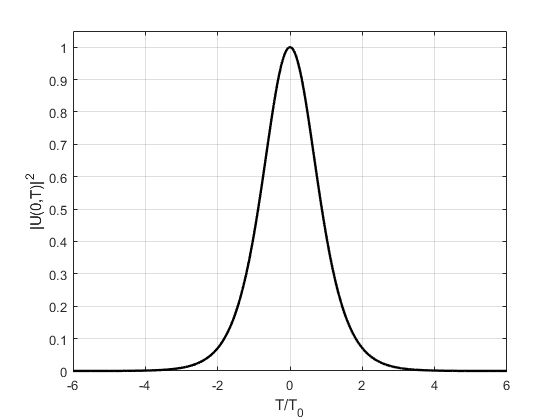
\includegraphics[width=0.6\linewidth]{figuras/PulsoHiperbolico.png}
  \caption{Envolvente temporal normalizada de un pulso hiperbólico-secante en el origen de la propagación con $C=0$}
  \label{hiper_z0}
\end{figure}

\subsection{Frecuencia instantánea}
La frecuencia instantánea, $\omega_{\mathrm{inst}}(t)$, de un pulso se define como la frecuencia angular predominante en cada instante de tiempo y se obtiene directamente a partir de la fase temporal. En el caso más general, se puede expresar como:
\begin{equation}
\omega_{\mathrm{inst}}(t) = \omega_{0} - \dfrac{d\phi(t)}{dt},
\end{equation}
donde $\omega_{0}$ es la frecuencia angular central del pulso y $\phi(t)$ la fase temporal. Esta formulación permite describir cómo evoluciona la frecuencia a lo largo del pulso: si la fase permanece constante, la frecuencia instantánea coincide con $\omega_{0}$; en cambio, si la fase varía con el tiempo, la frecuencia instantánea también cambia, dando lugar al fenómeno conocido como \textit{chirp} \cite{Trebino}.

En esta sección se emplea $t$ como tiempo; cuando se use $T$, se referirá al tiempo retardado en el marco de la envolvente.

\subsection{\textit{chirp}}
El \textit{chirp} aparece cuando la frecuencia instantánea de un pulso no permanece constante, sino que varía progresivamente a lo largo del tiempo. Este fenómeno puede aparecer de diferentes formas: de manera natural en la propia fuente emisora (por ejemplo, en la modulación directa de diodos láser), como consecuencia de la propagación en medios dispersivos o debido a efectos no lineales como la autofase modulada. Asimismo, puede introducirse de forma intencionada mediante técnicas de modulación externa o sistemas ópticos de \textit{prechirp}, con el fin de compensar la dispersión acumulada durante la transmisión \cite{Agrawal,España}.

Un pulso con \textit{chirp} puede presentar dos comportamientos distintos según la evolución de su frecuencia instantánea. En el caso de un \textit{chirp} positivo, la frecuencia aumenta progresivamente con el tiempo, de modo que el pulso comienza con componentes de menor frecuencia y termina con las de mayor frecuencia \cite{Trebino} como se observa en la Figura~\ref{Figura7}.

\begin{figure}[H]
  \centering
  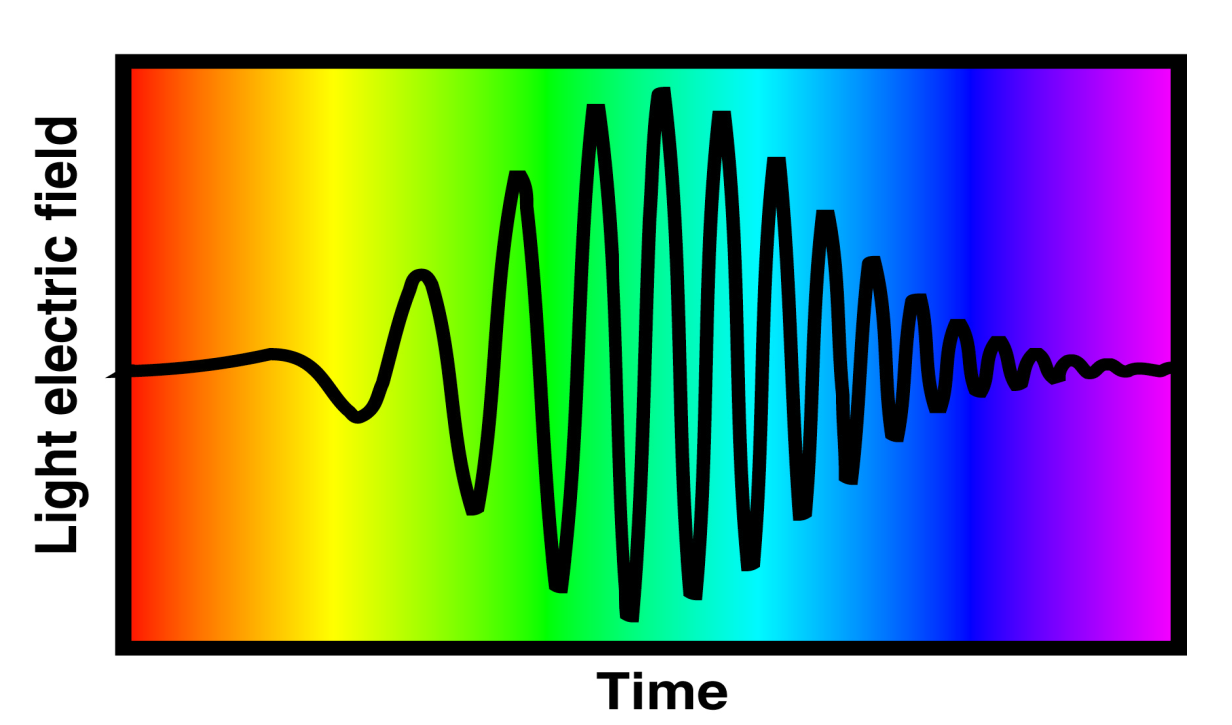
\includegraphics[width=0.7\linewidth]{figuras/Figura7.png} 
  \caption{Representación esquemática de un pulso con \textit{chirp} positivo. Fuente:~\cite{Trebino}}
  \label{Figura7}
\end{figure}

Por el contrario, con \textit{chirp} negativo, la frecuencia instantánea disminuye con el tiempo, de manera que el pulso empieza dominado por las frecuencias altas y finaliza con las bajas \cite{Trebino} como se observa en la Figura~\ref{Figura8}.

\begin{figure}[H]
  \centering
  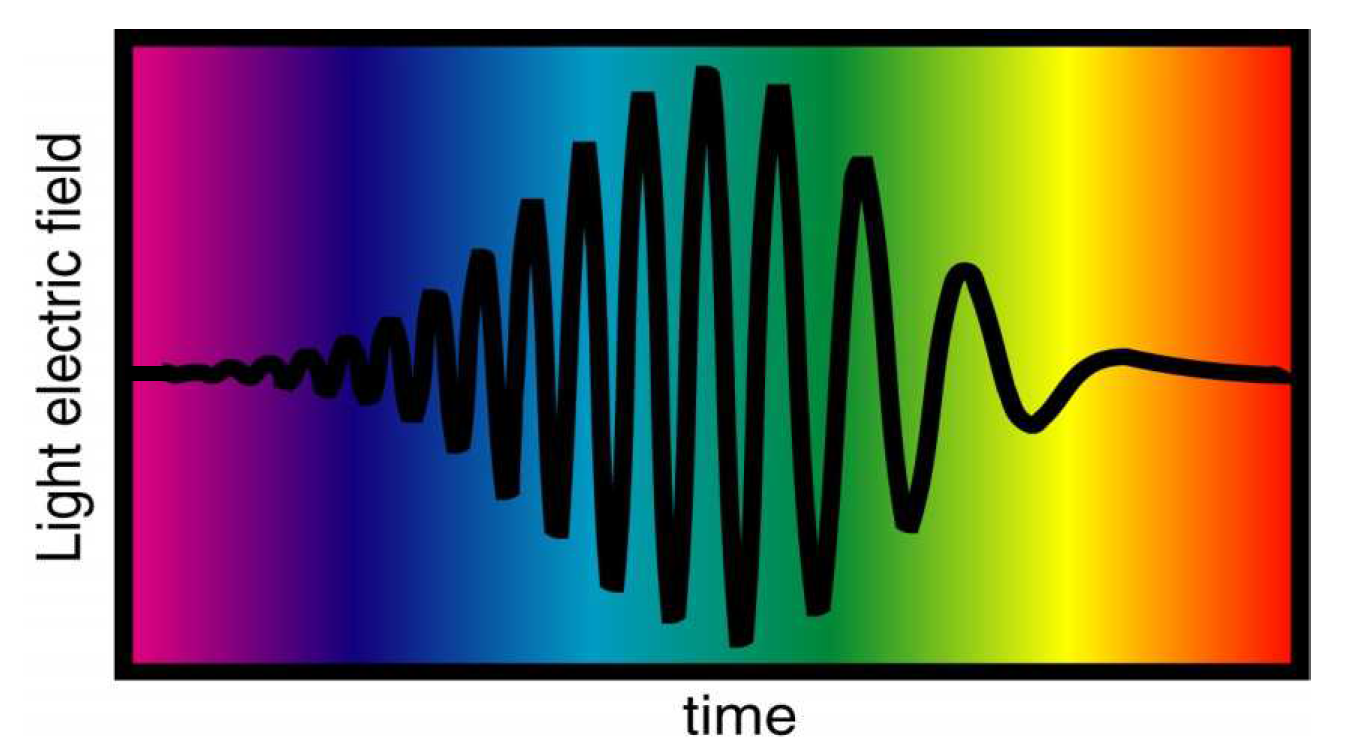
\includegraphics[width=0.7\linewidth]{figuras/Figura8.png} 
  \caption{Representación esquemática de un pulso con \textit{chirp} negativo. Fuente:~\cite{Trebino}}
  \label{Figura8}
\end{figure}

\subsection{Velocidad de grupo y retardo de grupo}
En transmisiones ópticas, una onda real no es perfectamente monocromática, sino que está formada por un conjunto de frecuencias próximas. En este contexto, no es suficiente con emplear la velocidad de fase, que solo describe el avance de la portadora, sino que resulta más adecuado introducir la velocidad de grupo.

Cuando una portadora de frecuencia $\omega_{0}$ es modulada por una envolvente $f(t)$, la portadora se propaga a la velocidad de fase, mientras que la envolvente lo hace a una velocidad distinta, denominada velocidad de grupo ($v_\mathrm{g}$). Esta magnitud describe el avance del pulso como conjunto y se define como:
\begin{equation}
v_\mathrm{g} = \left( \frac{d\beta}{d\omega} \right)^{-1},
\end{equation}
donde $\beta$ es la constante de propagación y $\omega$ la frecuencia angular.
El retardo asociado al pulso al propagarse una distancia $L$ recibe el nombre de retardo de grupo ($\tau_\mathrm{g}$) y se expresa, de acuerdo con \cite{España}, como:
\begin{equation}
\tau_\mathrm{g} = \frac{L}{v_\mathrm{g}}.
\end{equation}


\subsection{Dispersión (\textit{scattering})}
En óptica, el término dispersión puede referirse también al fenómeno conocido como \textit{scattering}, es decir, el esparcimiento de la luz en múltiples direcciones al propagarse por un medio transparente. Este efecto se produce cuando la onda encuentra imperfecciones o variaciones microscópicas del índice de refracción en el material, como ocurre en la atmósfera, en la fibra óptica o en el océano. Una consecuencia de este proceso es la atenuación de la señal, ya que parte de la energía luminosa se redistribuye en modos distintos al modo original, muchos de los cuales se pierden al no quedar confinados en el medio \cite{España}.

Es importante diferenciar este fenómeno del concepto de dispersión cromática, que se refiere al ensanchamiento temporal de un pulso cuando sus distintas frecuencias se propagan a velocidades diferentes. En cambio, el \textit{scattering} se produce por el desvío de la luz al interactuar con moléculas o partículas del medio, un proceso que depende tanto de la longitud de onda como del tamaño de dichas partículas. Mientras que el \textit{scattering} redistribuye la luz en múltiples direcciones, la dispersión cromática se vincula a la distorsión temporal que experimentan los pulsos.

\subsection{Dispersión cromática y coeficiente de dispersión}
La dispersión cromática, también denominada dispersión intramodal, tiene su origen en la dependencia no lineal de la constante de propagación con la frecuencia \cite{España}. En el contexto de este trabajo, al referirse a la constante de propagación se considerará exclusivamente la constante de fase, ya que la atenuación no altera la forma temporal de los pulsos y el interés se centra en los efectos dispersivos que afectan a pulsos ultracortos.

La constante de propagación está directamente relacionada con el índice de refracción del medio, según la expresión:
\begin{equation}
\beta(\omega) = \frac{\omega n(\omega)}{c}.
\end{equation}
Dado que el índice de refracción, $n(\omega)$, no es constante, sino que varía con la frecuencia, la relación entre $\beta$ y $\omega$ resulta no lineal. Este efecto provoca que las distintas componentes espectrales de un pulso ultracorto viajen a velocidades distintas, lo que genera retardos diferenciales y un ensanchamiento temporal del pulso.

Cuando una señal óptica modulada se transmite, suele ser cuasimonocromática, estando centrada en una frecuencia central $\omega_{0}$ y presentando pequeñas desviaciones $\Omega$. Así, cada componente espectral se propaga con su propia constante de propagación, donde $\omega = \omega_{0} + \Omega$. En un medio no dispersivo, todas las frecuencias se propagarían con la misma $\beta$, pero en medios dispersivos (siendo ese el caso de estudio en este trabajo), cada frecuencia experimenta una velocidad distinta deformándose así la forma del pulso.

Dado que las desviaciones en frecuencia respecto a la portadora son pequeñas, se puede aproximar la constante de propagación mediante un desarrollo en serie de Taylor alrededor de la frecuencia central como:
\begin{equation}
\beta(\omega) \approx \beta_{0} + \beta_{1}(\omega - \omega_{0}) + \frac{1}{2}\beta_{2}(\omega - \omega_{0})^{2} + \frac{1}{6}\beta_{3}(\omega - \omega_{0})^{3} + \dotsb
\end{equation}
Cada coeficiente de esta expansión tiene un significado físico concreto:
\begin{itemize}
  \item $\beta_{0}$: constante de propagación en la frecuencia central.
  \item $\beta_{1}$: determina el retardo con el que se desplaza la envolvente del pulso.
  \item $\beta_{2}$: coeficiente de dispersión cromática, también denominado \acs{GVD}~(\acl{GVD}).
  \item $\beta_{3}$: coeficiente de dispersión de tercer orden, también denominado \acs{TOD}~(\acl{TOD}). 
\end{itemize}


Además del coeficiente $\beta_{2}$, es habitual caracterizar la dispersión cromática de un medio mediante el denominado coeficiente de dispersión, $D$. Consiste en un parámetro característico de los medios dispersivos. Se emplea habitualmente porque ofrece una interpretación práctica: indica la diferencia de retardo temporal entre dos componentes espectrales cercanos de un pulso al propagarse por una distancia determinada \cite{España}. 

Tanto $D$ como $\beta_{2}$ cuantifican el ensanchamiento temporal de los pulsos ópticos, pero desde marcos de referencia distintos: el primero respecto a longitudes de onda y el segundo respecto a frecuencias.

\section{Turbulencia óptica}

En esta sección se presenta el fenómeno físico de la turbulencia óptica y se describen las herramientas matemáticas empleadas para modelarlo. El objetivo es introducir los fundamentos necesarios para su tratamiento posterior. Se explican las causas y características de las fluctuaciones del índice de refracción y los modelos estadísticos utilizados para representarlas, como la función de coherencia mutua y la irradiancia promedio, que permiten cuantificar su impacto. 

Estos elementos constituyen la base teórica que se empleará en el capítulo siguiente para analizar de forma detallada cómo la turbulencia, combinada con la dispersión cromática, afecta a la evolución temporal de los pulsos ópticos en medios atmosféricos y oceánicos.

Tanto la atmósfera como el océano presentan irregularidades que distorsionan el frente de onda, generan fluctuaciones de intensidad y provocan ensanchamiento temporal adicional. Para describir estos fenómenos se emplean modelos estadísticos basados en espectros de potencia y herramientas como la función de coherencia mutua y la irradiancia promedio, que permiten caracterizar cuantitativamente el efecto de la turbulencia en la propagación del pulso.

\subsection{Descripción general de la turbulencia óptica}
La turbulencia óptica se entiende como el conjunto de fluctuaciones aleatorias del índice de refracción presentes en un medio, que alteran la propagación de un haz óptico al introducir distorsiones de fase y variaciones de intensidad. Estos cambios afectan directamente a la forma temporal y espacial del pulso, provocando efectos como ensanchamiento adicional, centelleo o \textit{scintillation}, desplazamiento del haz y pérdida de coherencia.

Aunque su origen físico difiere entre la atmósfera y el océano, variaciones térmicas en un caso y gradientes de temperatura, salinidad o presión en el otro, los efectos ópticos resultantes son análogos. En ambos medios, las fluctuaciones del índice de refracción pueden describirse mediante modelos espectrales que caracterizan la intensidad de la turbulencia en función de la escala espacial. Asimismo, herramientas estadísticas como la función de coherencia mutua y la irradiancia promedio permiten cuantificar el impacto de estas fluctuaciones sobre la propagación del pulso.

\subsection{Turbulencia atmosférica}
La turbulencia atmosférica surge como consecuencia de variaciones aleatorias de temperatura en el flujo de aire, generando celdas con índices de refracción distintos. Cuando un pulso óptico atraviesa estas regiones irregulares, sufre aberraciones que distorsionan la onda y producen fluctuaciones de intensidad, degradando la calidad de la señal recibida\cite{Trichili}.  


La estructura de la turbulencia se caracteriza mediante dos escalas principales: la escala interna ($l_0$), del orden de milímetros y asociada a las irregularidades más pequeñas; y la escala externa ($L_0$), del orden de metros, que representa remolinos de mayor tamaño \cite{Andrews}. La turbulencia a pequeña escala está directamente relacionada con el centelleo, mientras que las inhomogeneidades de gran tamaño producen desplazamientos del haz en la apertura del receptor \cite{Trichili}.

Su descripción estadística se basa en el espectro de potencia de las fluctuaciones del índice de refracción. El modelo más extendido es el espectro de Kolmogorov,
\begin{equation}
\Phi_{n}(\kappa) = 0.033\, C_{n}^{2}\, \kappa^{-11/3},
\end{equation}
donde $C_n^2$ es el parámetro estructural del índice de refracción. Una formulación más realista es el espectro de von Kármán modificado, 
\begin{equation}
\Phi_{\mathrm{MVK}}(\kappa) = 0.033\, C_{n}^{2}\, 
\exp\left(-\frac{\kappa^{2}}{\kappa_{m}^{2}}\right)
\left(\kappa^{2} + \kappa_{0}^{2}\right)^{-11/6},
\end{equation}
con $\kappa_m = 5.92/l_0$ y $\kappa_0 = 2\pi/L_0$ \cite{Trichili}.



Finalmente, la intensidad de las fluctuaciones inducidas por la turbulencia atmosférica se clasifica habitualmente en función de la fuerza de las fluctuaciones de irradiancia. Para distinguir entre los distintos regímenes de turbulencia se emplea la varianza de Rytov, que constituye una medida fundamental de la intensidad de la turbulencia atmosférica. La varianza de Rytov se define como:
\begin{equation}
\sigma_R^2 = 1.23\, C_n^2\, k^{7/6}\, L^{11/6},
\end{equation}
donde $C_n^2$ es el parámetro estructural de las fluctuaciones del índice de refracción, $k = 2\pi/\lambda$ es el número de onda y $L$ es la distancia de propagación \cite{Phillips}.

Cuando $\sigma_R^2 \ll 1$, el canal atmosférico se encuentra en el régimen de turbulencia débil, caracterizado por fluctuaciones suaves de la irradiancia. Para valores $\sigma_R^2 \gtrsim 1$, las fluctuaciones se vuelven moderadas o fuertes, dando lugar a fenómenos más severos. En este último caso, el régimen suele denominarse turbulencia fuerte o profunda.\cite{Phillips}

Además de la varianza de Rytov, existen métricas complementarias que permiten evaluar la degradación de la señal en recepción, como el \acs{SR}~(\acl{SR}), relacionado con la degradación del frente de onda, y el índice de \textit{scintillation} ($\sigma_I^2$), que cuantifica las fluctuaciones de intensidad inducidas por la turbulencia atmosférica \cite{Trichili}.


\subsection{Turbulencia oceánica}
La turbulencia oceánica se define como un movimiento aleatorio e irregular del fluido caracterizado por remolinos que mezclan calor, sal y energía cinética \cite{Sun}. Las fluctuaciones del índice de refracción en el agua se originan principalmente por gradientes de temperatura, salinidad y presión, además de la posible presencia de burbujas de aire. Estas irregularidades modifican la propagación del haz óptico, generando distorsiones, fluctuaciones de intensidad, desplazamiento del haz, variaciones en el ángulo de llegada, moteado y pérdida de coherencia \cite{Baykal}.

La turbulencia oceánica presenta una marcada dependencia espectral: las longitudes de onda de la ventana azul-verde sufren menor absorción y permiten mayor alcance, pero también resultan más sensibles a la turbulencia; mientras que las longitudes de onda más largas, como el rojo o el infrarrojo cercano, muestran mayor absorción pero menor sensibilidad a estas fluctuaciones \cite{Sun}.

Según la homogeneidad y dirección del flujo, la turbulencia puede clasificarse en isotrópica o anisotrópica. En trayectorias horizontales poco profundas y con salinidad moderada, suele asumirse isotropía y homogeneidad \cite{Ata}. 

Los parámetros físicos que más influyen en la intensidad de la turbulencia son:

\begin{itemize}
    \item \textbf{Salinidad}: incrementos en la salinidad aumentan la densidad del agua y refuerzan la turbulencia cuando domina su contribución espectral.
    \item \textbf{Temperatura}: determina la energía interna del fluido y condiciona la estratificación; cuando la temperatura domina, la turbulencia es más débil\cite{Thorpe,Thorpe2}.
    \item \textbf{Tasa de disipación de energía cinética turbulenta} y 
    \textbf{tasa de disipación térmica}: controlan la escala y la intensidad del movimiento turbulento \cite{Woods,Matt}.
\end{itemize}

Para describir cuantitativamente estas fluctuaciones se emplean modelos espectrales como:

\begin{itemize}
    \item \textbf{Nikishov-Nikishov}, que combina los espectros de temperatura, salinidad y su co-espectro. En este modelo, el espectro de potencia se expresa como \cite{Nikishov}:
    \begin{equation}
\Phi_n(\kappa) = A^2 \, \Phi_T(\kappa) 
+ B^2 \, \Phi_S(\kappa)
- 2AB \, \Phi_{TS}(\kappa),
\end{equation}
donde $\Phi_T(\kappa)$ y $\Phi_S(\kappa)$ representan los espectros de las fluctuaciones de temperatura y salinidad, respectivamente, y $\Phi_{TS}(\kappa)$ su co-espectro.
    \item \textbf{Hill (H4)}, aplicable a fluidos estratificados y que distingue rangos viscoso-conectivo, inercial y de disipación \cite{Hill}.
    \item \textbf{\acs{OTOPS}~(\acl{OTOPS})}, que generaliza modelos anteriores incorporando dependencia con temperatura media, salinidad y longitud de onda \cite{Korotkova}.
    \item Modelos posteriores, como el de Li, que incluyen efectos de estratificación y escala externa, o aproximaciones más precisas para los regímenes viscoso e inercial \cite{Li,Yi}.
\end{itemize}

\subsection{Herramientas estadísticas}
El análisis de la propagación de pulsos ópticos en medios turbulentos requiere herramientas que permitan describir de forma estadística cómo las fluctuaciones del índice de refracción afectan a la coherencia y a la intensidad de la señal. Entre ellas, destacan la función de coherencia mutua y la irradiancia promedio, que constituyen las bases matemáticas para caracterizar el ensanchamiento temporal y las fluctuaciones de intensidad inducidas por la turbulencia tanto atmosférica como oceánica.

\subsubsection{\acs{MCF}~(\acl{MCF})}
La MCF es una herramienta fundamental para describir cómo se correlacionan las distintas componentes espectrales de un pulso óptico tras propagarse por un medio aleatorio. Proporciona una medida directa del ancho de banda de coherencia y del tiempo de coherencia del pulso.

Se define matemáticamente como el promedio estadístico del producto del campo eléctrico complejo en una posición y frecuencia con el conjugado de ese mismo campo en otra posición y frecuencia \cite{Ronald}:
\begin{equation}
\Gamma_{2}(r_{1}, r_{2}, L; \omega_{1} + \omega_{0}, \omega_{2} + \omega_{0}) = 
\langle U(r_{1}, L; \omega_{1} + \omega_{0}) \, U^{*}(r_{2}, L; \omega_{2} + \omega_{0}) \rangle,
\end{equation}
donde $\Gamma_{2}$ es la función de coherencia mutua, $r_{1}$ y $r_{2}$ representan las posiciones espaciales, $L$ la distancia de propagación, $\omega_{0}$ la frecuencia central del pulso, $\omega_{1}$ y $\omega_{2}$ las desviaciones respecto a $\omega_{0}$, $U(r, L; \omega)$ el campo eléctrico complejo, $\langle \cdot \rangle$ el promedio estadístico y $^{*}$ el conjugado complejo.

\subsubsection{Irradiancia promedio}
La irradiancia se refiere específicamente a la energía que llega a una superficie con una orientación concreta \cite{Paschotta}. En un medio aleatorio como la atmósfera turbulenta o el océano, la irradiancia instantánea no es determinista, sino que experimenta fluctuaciones debidas a los efectos del medio.

Para caracterizar su comportamiento se introduce la irradiancia promedio, entendida como el valor esperado estadístico de la irradiancia instantánea. Su formulación se obtiene directamente a partir de la MCF, lo que permite vincular la irradiancia con la correlación espectral del pulso. De este modo, constituye una magnitud fundamental para analizar el ensanchamiento temporal en medios turbulentos \cite{Ronald}.

Matemáticamente, la irradiancia promedio para un pulso óptico gaussiano viene dada por:
\begin{equation}
\begin{aligned}
&I(r, L; t) = \frac{T_0^2}{4\pi} \int_{-\infty}^\infty \int_{-\infty}^\infty 
 \exp\left(-\frac{1}{2} \omega_c^2 T_0^2 \right)
\exp\left( -\frac{1}{8} \omega_d^2 T_0^2 \right) \\
& \Gamma_2\left(r, r, L; \omega_0 + \omega_c + \frac{1}{2}\omega_d,\, \omega_0 + \omega_c - \frac{1}{2}\omega_d\right)
\exp(-i\omega_d t)\, d\omega_c\, d\omega_d,
\end{aligned}
\end{equation}
donde $I(r, L; t)$ representa la irradiancia promedio en la posición $r$, a una distancia $L$ y en el instante $t$, $T_0$ es la duración característica del pulso, $\Gamma_2$ es la MCF, $\omega_c$ es la frecuencia promedio y $\omega_d$ la diferencia de frecuencias \cite{Phillips}.





\chapterend{}
